\chapter{图的遍历、分解与简化}
\label{chap:graph-traversal}

第13章把“存在一条路径”“两点被条件集分离”这些判据定义清楚了。本章让它们变得可执行：
在一张真实的、可能有上百万顶点的图上，怎样真正列出可达点、检出回路、排出执行次序、
给连通区域编号、抽出连接骨架、沿少数接口把大图拆成可分别计算的局部块，
以及怎样把一次d-分离查询变成一次普通的无向可达查询。

这些操作输出的对象不同：遍历输出访问次序与发现路线，连通标记输出分量编号，
骨架提取输出一组边，分块与\term{树分解}输出局部袋和它们之间的接口，
d-分离判定则只输出“分离/不分离”以及一条证据。先确定要输出什么，再选择保存什么状态，
不能因为它们都要“沿边走一遍”就当成同一算法。

本章默认输入是有限图及其邻接表，仍排除自环和平行边；放宽时会另行保存边身份。
记顶点数为$n$、无向边数为$m$、有向弧数为$a$。无向边在邻接表中从两端各存一次，
需要逆向检索时还要另建一份入邻接表，其建立时间与存储都要计入。
图上的\term{消元}只负责组织潜在的中间作用域；至于中间表上的数值能否合法组合、汇总，
要到第16章的配置查询才解决，本章不预设其运算正确。

\section{基于队列与栈的图遍历法}

两种最基础的遍历都沿邻接表枚举邻居，区别在于等待处理的顶点按什么次序取出。

\paragraph{队列}
队列先进先出：较早发现的顶点先被取出，后来的顶点排在队尾。这种次序适合由近及远、
按距离起点的层数展开，具体的距离状态在广度遍历中建立。

\paragraph{栈}
栈后进先出：最后加入的元素先取出，可以保存一条尚未走完的当前分支。
深入时压入新顶点，走到底再弹出已完成顶点。深度遍历仅靠“后进先出”还不够，
每一帧还要记录下一条尚未检查的邻边位置，否则无法正确恢复分支。

\paragraph{遍历方法的输出}
广度遍历主要保存距离层与一条发现路线，深度遍历保存当前分支、回边与完成信息。
后面的连通标记、拓扑排序和骨架提取都会复用其中一种遍历，但各自只取所需结果。

\subsection{基于队列的广度优先遍历法}
\label{sec:graph-theory-bfs}

\paragraph{按层扩展的思想与状态}
给定起点$s$，要列出所有可达点并为每点保留一条到达路线，
可以先查一跳邻居、再查两跳邻居，而不必枚举所有完整路径。
\term{广度优先搜索}（breadth-first search, BFS）用队列维持这个由近及远的次序。
状态包括发现标记、队列$Q$、边数距离$d$和父指针$p$：
初始只标记$s$，令$d(s)=0$、$p(s)$为空并把$s$入队，其余点距离记$+\infty$。
这里度量的是边数，边权不参与。

\paragraph{入队标记与逐步实现}
\begin{algorithm}[基于队列的广度优先遍历]
  队列非空时取出队首$u$，逐个读取其邻居$v$（有向图只读取出邻居）。
  若$v$尚未发现，立即把它标记为已发现，置$d(v)=d(u)+1$、$p(v)=u$并入队；
  全部邻居处理完后继续下一个队首，直到队列为空。
\end{algorithm}
标记必须发生在入队时，而不是出队时：两个已发现点可能共享一个尚未发现的邻居，
若等出队才标记，同一点会被重复加入队列。对不可达点保留$+\infty$，
不把“没访问到”误解为该点是孤立点。需要路线时，从已发现的终点沿父指针逆向回到$s$再反转；
父指针总指向更早发现的点，因而不会成环。

\paragraph{贯穿图的队列轨迹}
约定邻居按编号递增访问，从$1$出发：队列初始为$[1]$；取$1$后变为$[2,3]$；
取$2$时发现$4$，变为$[3,4]$；取$3$时$4$已发现，不重复入队；取$4$后队列为空。
同时记录$d(2)=d(3)=1$、$d(4)=2$，父指针$p(4)=2$，恢复路线$1-2-4$。
若邻居访问次序改变，$4$的父亲也可能是$3$，路线不同但距离仍是$2$。

\paragraph{基本分析与选择边界}
队列在处理第$k$层时才会首次加入第$k+1$层的点。归纳地，若更早层距离都正确，
处理第$k$层时新发现的邻居必有一条长度$k+1$的路径；若它还有更短路径，
其倒数第二个点会在更早层被处理并更早发现它，矛盾。因此首次记录的层数就是最少边数，
而不只是“逐层”这个名称带来的直觉。每个顶点至多入队一次，每条边或弧检查常数次，
邻接表下时间为$O(n+m)$（有向图为$O(n+a)$），标记、距离、父指针与队列占$O(n)$额外空间。
若改用稠密矩阵逐行扫描邻居，不能沿用这一代价。边长不全相等时，
最少边数也不等于最低累计成本，那要使用第15章的带权最短路方法。

\subsection{基于栈的深度优先遍历法}
\label{sec:graph-theory-dfs}

\paragraph{保持当前分支的思想与状态}
若要系统地查找回路，就要沿一条未完成分支持续深入、走到尽头再退回。
\term{深度优先搜索}（depth-first search, DFS）按这种方式访问未探索邻居。
顶点分为未发现、在栈内、已完成三种状态，以区分“第一次抵达”与“已处理完全部邻居”。
采用显式栈时，每帧保存顶点$u$以及该帧下一条待查邻边的位置，另存父指针和完成序列。

\paragraph{深入、回退与回边恢复}
\begin{algorithm}[基于显式栈的深度优先遍历]
  选一个未发现起点，标记为在栈并压入首帧。查看栈顶的下一条邻居$v$并推进该帧的邻边位置：
  $v$未发现时记父指针、改为在栈并压入新帧；$v$在栈内时这是一条回边；$v$已完成则继续看下一条。
  栈顶所有邻居耗尽后，把它改为已完成、记入完成序列并弹栈。栈空后若要遍历全图，
  另选尚未发现的起点重复，已完成点不重新初始化。
\end{algorithm}
有向图中$u\to v$指向栈内顶点时，父指针已保存$v$到$u$的栈内有向路径，连同该弧构成有向环，
沿父指针恢复即可得到一个环见证。无向图要跳过实际的父边，不能把同一树边的反向查看当成环；
允许平行边时按边身份只跳过那一条父边。指向已完成点的弧不提供当前分支成环的证据。

\paragraph{三点分支的执行轨迹}
在有向三角$1\to2\to3\to1$上，栈依次为$[1]$、$[1,2]$、$[1,2,3]$；
检查$3\to1$时$1$仍在栈，沿父指针得$3\leftarrow2\leftarrow1$，补回$3\to1$即恢复该环。
删去$3\to1$后，$3$先耗尽邻居出栈，再完成$2,1$，完成序列为$3,2,1$。

\paragraph{基本分析与输出比较}
若存在有向环，沿环的完成先后关系不可能处处严格前进，DFS必遇到指向尚未完成顶点的回边，
这与上面的环见证合起来给出有向判环的双向依据。每点进栈、出栈各一次，
每条邻边检查常数次，时间为$O(n+m)$（或$O(n+a)$），状态与栈占$O(n)$，栈深最坏为$n$；
显式栈避免把很长路径直接交给语言递归栈。无向图中从未访问点重启可得到各连通分量，
但有向图这样得到的只是访问森林，不能当作强连通分量。DFS也不保证发现路线边数最少。

\section{无环依赖下的拓扑排序法}
\label{sec:graph-theory-topological-order}

依赖图要求每条弧的起点先于终点处理，否则就会用到尚未算出的结果。
满足这一要求的顶点排列称为拓扑序：它把“谁必须先于谁”的偏序扩展成可逐个执行的线性次序；
没有直接边的两点仍可能通过一条长路径互相依赖。

\paragraph{排序的输入条件与输出}
方法接收一个有限有向图：成功时返回覆盖全部顶点的一个拓扑序，失败时报告有环。
有限有向图存在拓扑序当且仅当它不含有向环——若有环
$v_1\to v_2\to\cdots\to v_k\to v_1$，次序既要求$v_1$先于$v_2$、一路到$v_k$，
又要求$v_k$先于$v_1$，矛盾；反之DAG总能找到入度为零的顶点，删去后余图仍是DAG，反复即可排完。
下面给出两种构造，存在性结论本身不是第三种算法。

\subsection{基于零入度队列的Kahn排序法}

\paragraph{删除已无前驱的任务}
当前没有未完成前驱的点可以安全输出。若非空有限图处处仍有前驱，
沿前驱反向追溯必会在有限顶点中重复，重复段按原弧方向构成有向环；
因此DAG每一步都能找到下一个零入度点。状态是当前入度数组、零入度队列和输出序列；
入度必须对应尚未删除的图，不能始终用初始入度判断。

\paragraph{初始化与逐弧减度}
\begin{algorithm}[Kahn拓扑排序]
  扫描全部弧统计初始入度，把所有零入度点（包括孤立点）入队。
  取出$u$追加到输出末尾，对每条弧$u\to v$把$v$的当前入度减$1$，恰降为$0$时才入队。
  队列空时结束：输出了$n$个点则得到拓扑序，不足$n$个说明剩余点都没有零入度入口，报告有环。
\end{algorithm}
一条弧总在其起点输出后才从终点入度中扣除，因此每条依赖都得到满足；
不能把已输出的前缀冒充完整排序。

\paragraph{菱形依赖的轨迹与分析}
在$1\to2$、$1\to3$、$2\to4$、$3\to4$上，初始入度为$(0,1,1,2)$。
取$1$后$2,3$入队；取$2$只把$4$的入度降为$1$；取$3$才把$4$降为$0$并入队，
输出$1,2,3,4$。每弧减度一次、每点入队一次，邻接表下时间$O(n+a)$、额外空间$O(n)$。
队列中并列的零入度点任选其一，会得到不同但都合法的序列；
若为了复现而按编号优先选点，要另计优先队列的代价。

\subsection{基于DFS逆完成序的拓扑排序法}

\paragraph{从分支完成次序构造}
直接复用深度遍历的三色状态与完成序列，同时检查有向回边。图无回边时，对任意弧$u\to v$：
查看时$v$若未发现，会作为递归后继先于$u$完成；若已完成，本就更早完成；
$v$在栈内的情形已被无环条件排除。因此每条弧都从较晚完成者指向较早完成者，
把完成序列反转便得到拓扑序。

\begin{algorithm}[DFS逆完成序拓扑排序]
  覆盖全部顶点执行DFS；一旦发现回边就返回环见证并拒绝输出；
  否则把完整完成序列反转。不能只对一个起点的可达区反转后就声称排好了全图。
\end{algorithm}

\paragraph{同图比较与边界}
在同一菱形图上按编号探索，从$1$经$2$到$4$，完成$4,2$，再经$3$完成$3,1$，
反转得到$1,3,2,4$。它与Kahn可能给出的$1,2,3,4$不同，但逐条弧检查都满足依赖。
两法都为$O(n+a)$，区别只在维护入度队列还是分支栈：需要持续列出当前可执行任务时Kahn更直接，
已经需要DFS的环见证与完成信息时逆完成序可直接复用。
注意只有在拓扑序中相邻且互相不可达的两个顶点才能交换；
仅有边$a\to b$和孤立点$c$时，$(a,b,c)$合法，但交换不相邻的$a,c$得到$(c,b,a)$就破坏了依赖。

\section{基于邻接检索与标签合并的连通标记法}

给网格或一般图的每个连通区域一个编号，是遍历的直接应用。先固定两类不同输入：
哪些位置属于前景，以及前景位置之间允许怎样相邻。

\paragraph{前景位置集合}
网格数组先用指定数值或掩模选出前景位置，标记只处理这些位置。
“位置是否属于前景”与“两个位置是否相邻”是两项独立输入，不能由同一个数组值自动推出。

\paragraph{4邻接与8邻接}
二维位置$(i,j)$的4邻域是上下左右四个位置；8邻域再加入四个对角位置。
只保留两端都是前景的边。若前景只有$(0,0)$、$(1,1)$两点，4邻接下它们分属两个分量，
8邻接下则因角相接而同属一个分量。一次标记必须自始至终使用同一套已固定的邻接规则。

\paragraph{分量标签与种子可达标记}
用同一编号标记一个连通分量中的全部前景位置，不同分量用不同编号。
一般无向图直接使用给定邻接表，网格则结合前景与邻域形成允许边。
若只关心与指定起点集合相连的位置，可以只标记其可达区域而不为其余分量编号，这称为种子可达标记。

\subsection{基于BFS重启的分量标记法}

\paragraph{一次标记一个可达区域}
状态为未标记/分量编号数组、下一个分量号和队列。扫描全部位置，
每遇到一个尚未标记的前景点就启动一次BFS，把这次新发现的点都赋同一编号；
一次队列清空后再寻找下一个起点，旧编号保留不清除。
\begin{algorithm}[重启BFS分量标记]
  对外层扫描到的每个未标记前景点，分配新分量号，从它启动BFS：
  取出队首位置，把符合前景与邻接规则、尚未标记的邻居标为当前分量号并入队；
  队列空后继续外层扫描。背景位置保持预定的背景标记。
\end{algorithm}

\paragraph{数例与基本分析}
只有$(0,0)$、$(1,1)$两个前景点时，4邻接下启动两次、得到两个编号，
8邻接下只启动一次、两点同号。邻接规则的差别正体现为检查到的候选边不同。
一般无向图总时间为$O(n+m)$；$P$个位置、固定局部邻域的网格为$O(P)$，
标记与队列最坏占$O(P)$空间。扫描顺序可能改变标签的字面值，但不改变分量这一划分。

\subsection{基于并查集的两遍扫描标记法}

\paragraph{临时标签的等价类}
按行读取数组时，两个临时标签可能在后面被发现属于同一区域，
需要保存“它们同类”而不必立即重写所有旧点。这种同类关系还须传递：
标签$1$与$2$同类、$2$与$3$同类，则三者最终归同一类。

\paragraph{并查集}
\term{并查集}维护这些标签的等价类：find返回类代表，union把两个类合并。
其内部父指针只维护标签之间的等价，不是原图上的空间边；第二遍扫描凭类代表决定最终标签。

\paragraph{先给临时标签再合并的思想}
第一遍只检查已经扫描过的邻居：4邻接查左、上，8邻接再查左上、右上。
没有已标记的前景邻居就新建一个临时标签；否则借用其中一个标签，
并把这次相遇的全部邻居标签用union合并。

\paragraph{两遍实现与区域重逢数例}
\begin{algorithm}[两遍扫描标记]
  第一遍逐行扫描，生成临时标签并union所有相遇的标签类；
  第二遍把每个位置的临时标签替换成其find代表，必要时再对代表统一连续编号。
\end{algorithm}
以前景三行
\[
  \begin{matrix}1&0&1\\1&0&1\\1&1&1\end{matrix}
\]
并固定4邻接为例：上方两支分别暂标$1,2$，扫描到第三行右端时，
左邻标签$1$与上邻标签$2$相遇而被合并，第二遍整片前景取同一代表。
每条网格边都在其较晚端点被考虑，等价关系的传递闭包恰好等于真正的连通关系；
暂时隔着背景的两支可能在后面重逢，不能把首遍编号永久当作不同分量。

\paragraph{代价与方法比较}
路径压缩加按秩合并时，$P$个位置的总摊还代价为$O(P\alpha(P))$，
其中$\alpha$是增长极慢的反Ackermann函数；另计标签与并查集的存储。
两遍扫描与重启BFS在相同邻接下输出相同的分量划分，差别只在数据访问方式与临时等价的维护，
不应为了比较而更换前景或$4/8$邻接规则。

\subsection{基于种子队列的掩模重建法}

\paragraph{掩模、种子与结构元}
有限位置集$G$规定允许访问的区域，称为掩模；扩张的每一步都必须留在$G$中，
画布上存在但不属于$G$的位置不能当作过桥的跳板。初始已标记位置集$F\subseteq G$称为种子，
任务是求掩模内能由这些种子到达的区域；$F$可以含多个位置，也可以为空，
空种子时不能从掩模自身凭空启动。有限偏移集$B$中的步长规定允许的邻接，称为结构元：
$B=-B$时才是无向邻接，非对称$B$只给有向可达；零向量是否属于$B$还决定旧位置能否自动保留。

\paragraph{累计可达集的思想}
当$0\in B$时，逐轮结果写成
\begin{equation}
  R_0=F,\qquad R_{k+1}=(R_k\oplus B)\cap G,
  \label{eq:graph-mask-reconstruction}
\end{equation}
其中$R\oplus B=\{r+b:r\in R,\ b\in B\}$。含零向量保证$R_k\subseteq R_{k+1}$，旧位置保留。
对轮数归纳可知$R_k$恰为掩模内从种子沿允许步长至多走$k$步可达的位置；
有限集合加单调增加保证停止，至多$|G\setminus F|$次严格增加。
$B=-B$时，稳定结果就是与种子相交的全部无向分量之并。

\paragraph{队列实现与边界}
\begin{algorithm}[种子队列掩模重建]
  把全部种子标记并入队；每次只扩展新加入的点，把仍在$G$中、尚未标记且符合$B$的邻居加入；
  队列空即返回。空种子返回空集；若$F\not\subseteq G$应拒绝输入或先明确取交的约定。
\end{algorithm}
在位置$0$至$4$上取$G=\{0,1,2,4\}$、$F=\{0\}$、$B=\{-1,0,1\}$，
逐轮得到$\{0\}$、$\{0,1\}$、$\{0,1,2\}$后稳定，位置$4$因断开而不加入，
队列只处理$0,1,2$。固定有限结构元时这是$O(|G|)$量级；
若$B$不含零向量又不与旧集取并，集合可能缩小或交替，队列法计算的“曾经可达”累计集
不能无声等同于那种非单调迭代。

\section{基于发现父边的生成森林提取法}
\label{sec:graph-theory-spanning-skeleton}

\paragraph{生成树、生成森林与提取目标}
在一个无向连通分量中，覆盖该分量全部原顶点且无环的连接子图称为\term{生成树}（spanning tree）；
原图每个分量各取一棵生成树，合起来得到生成森林。这里是从实际原边中抽取连接骨架，
边权可以随所选边保留但不参与选择，因此不承诺总成本最小（那是第15章最小生成树的目标）。

\paragraph{只保存首次发现的连接}
\begin{algorithm}[发现父边抽取生成森林]
  对每个尚未访问的顶点选作根，启动一次BFS或DFS；每次首次发现$v$时，
  保存使它被发现的实际边$\{p(v),v\}$，重复遇到已访问点时不再加边。
  状态为全局发现标记、所选边表和分量数。
\end{algorithm}
每个新点恰通过一条父边接入，父亲早于孩子，所选边不可能成环；完整遍历又覆盖该分量，
所以输出确为生成树。若原图有$n$个顶点、$c$个分量，生成森林恰有$n-c$条边。
空顶点集输出空森林；$n>0$但无边时输出$n$棵单点树，不能把非连通图硬称为一棵全图生成树。
并查集内部的父指针不是原图边，输出应使用实际记录的父边表。

\paragraph{贯穿图抽取与丢失信息}
从$2$启动BFS、按编号发现$1,3,4$，保留$\{1,2\},\{2,3\},\{2,4\}$，
得到以$2$为中心的树，而忽略$\{1,3\},\{3,4\}$。原图$1$与$3$直接相邻，
抽取后却要经$2$走两步；原图没有割点，删去$2$后仍有$1-3-4$相连，树中的三叶却被分开。
可见保留分量连通不等于保留全部距离、环或分离关系。总时间为$O(n+m)$、额外$O(n)$；
BFS父树还保留从所选根出发的无权距离，DFS父树一般连这一点也不保证。

\section{基于给定分隔集的局部分块法}
\label{sec:graph-theory-separators}

\paragraph{给定候选分隔集与删除后的分量}
输入有限无向图和一个给定的真子集$S$，本方法用这份待检验的删除集构造分块，
不负责寻找最小分隔集。暂时删除$S$及其关联边，把余图分成连通分量$C_1,\ldots,C_r$；
不同$C_j$之间没有直接原边。若删除后只有一个分量，应报告$S$没有形成多侧拆分，
不能因为输入名叫“分隔集”就假定已经拆开。

\paragraph{共享接口与局部因子归属}
把接口加回各块，得到局部诱导块$\mathcal G[C_r\cup S]$。重复出现在多个块中的是同一个变量，
不是可以分别取值的多个副本。若还提供局部因子，每个作用域必须完整容纳进某一块，
并指定唯一归属；纯接口因子也只能归一个块，不能因它被多个块引用就重复计入。
\begin{algorithm}[删除、标记与加回接口]
  暂时屏蔽$S$及其关联边，用连通标记得到全部$C_j$；为每个分量输出诱导块$\mathcal G[C_r\cup S]$，
  保存公共接口的唯一身份及在各块中的引用；逐作用域把每个因子归入唯一一个能容纳它的块。
  若只剩一个分量则报告未形成多侧拆分。
\end{algorithm}

\paragraph{固定接口后分别处理的思想}
贯穿图两侧都需要变量$2,3$，硬拆成不相交两块会失去核对它们取值的位置；
保留同一接口赋值后，内部变量才能分别组织。小接口之所以省算，是因为同时处理的变量数决定表规模：
每变量$q\geq2$个取值时，$b$个变量的稠密联合表有$q^b$项，二十个二值变量已逾百万项。
但小接口不保证内部简单：两个大团只共用一个点时接口很小，团内仍需枚举大量配置，
所以还需要后面的多袋树分解。结构分块本身不推出概率独立，
那还要求局部函数组成可归一化的非负联合权重。

\paragraph{贯穿图验证与基本分析}
取$S=\{2,3\}$，删除后得到$\{1\}$、$\{4\}$两个分量，加回接口为$\{1,2,3\}$与$\{2,3,4\}$；
三元因子$\phi_{2,3,4}$完整放右块，接口因子$\phi_{2,3}$只归一侧。
删$1$或$4$余下三角形，删$2$或$3$余下路径，贯穿图既无割点也无桥（每条边都在一个三角形中），
但二点接口$\{2,3\}$有效。删除与标记为$O(n+m)$；若复制每块中的接口，
还要计$r|S|$及$r|E(S)|$的重复量，因子作用域读取与内部表计算另计。

\section{基于消元补边的树分解法}
\label{sec:graph-theory-tree-decomposition}

本节集中树分解所需概念，再比较给定次序与动态选次序两种构造。
概念用来核验输出，方法主体仍是补边、删点、记袋和连接父袋。

\subsection{树分解的基本概念}

\subsubsection{原图中的团与计算用袋}
两两相邻的顶点集合称为\term{团}（clique），检查的是原图中每对不同顶点之间是否有边，
不看画出来是否围成封闭区域；全部顶点构成团时称\term{完全图}。
贯穿图中$\{1,2,3\}$是团而$\{1,2,4\}$不是（缺边$1-4$）。
\term{袋}是准备放进同一个中间表里同时索引的变量集合；袋不必是原图的团——
补边消元产生的袋就可能含原图中不直接相邻的变量，不能把计算用袋等同于已有因子。
把袋作为新树的节点时，相邻两袋的交集称为接口，它保存共同变量的取值，
袋树边本身不是原图边。

\subsubsection{树分解与运行交集}
\begin{definition}[树分解]
  \label{def:graph-theory-tree-decomposition}
  有限无向图$\mathcal G=(V,E)$的树分解由一棵有限树$\mathcal T$和每个树节点$t$上的袋
  $B_t\subseteq V$组成，满足：每个原顶点至少进入一个袋；每条原边两端共同进入某个袋；
  对任一原顶点$i$，含$i$的全部袋在$\mathcal T$上连通。最后一条称为\term{运行交集性质}。
\end{definition}

\begin{figure}[htbp]
  \centering
  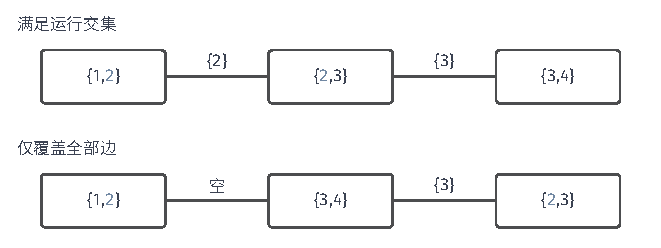
\includegraphics[width=112.0mm]{figures/01-mathematical-preliminaries-upper/05-graphs-and-signals/tikz/graph-theory-running-intersection/figure.pdf}
  \caption{同一四顶点路径的两种袋连接。上行依次连接
  $\{1,2\},\{2,3\},\{3,4\}$，既覆盖边，又让每个变量的出现位置连通。
  下行同样覆盖全部边，却把含$2$的两个袋隔开，中间袋无法携带$2$的取值，因而不是树分解。}
  \label{fig:graph-theory-running-intersection}
\end{figure}

如图~\ref{fig:graph-theory-running-intersection}，仅覆盖顶点和边还不够：
在路径$1-2-3-4$上，若把两个含$2$的袋用不含$2$的袋隔开，两端就能分别取$z_2=0$和$z_2=1$
而沿途无从核对。运行交集保证一个变量的出现位置连成连通子树，
相邻接口上的一致性可以传到它的全部出现位置。

\paragraph{团作用域的整袋容纳}
树分解中任意一个团都整体包含在某个袋里，因此原始图中成团的高阶作用域能完整入袋。
其依据是树上的Helly性质：树上若干棵两两相交的连通子树必有公共顶点。
对团$C$，每个顶点$v\in C$出现的袋集合由运行交集保证是连通子树，
而边覆盖又使团内任意两点的子树两两相交，于是这些子树共有某个装下整个$C$的袋。
结构上能容纳仍不等于数值查询正确：因子还要唯一归属，组合与汇总规则由第16章给出。

\subsubsection{顶点消元与填充}
想不再显式保留变量$v$，先要把所有含$v$的局部表的影响组织到剩余变量上。
图上的操作是：删除$v$前检查它当前的剩余邻居，必要时在邻居间补齐连接，再删去$v$及关联边。
新补的边称\term{填充边}（fill edge），它记录新表可能具有的联合索引，
不是原问题新增的独立约束；特殊函数有时仍可继续分解，袋给的是通用的作用域上限。

\subsubsection{分解宽度与树宽}
一个树分解的宽度是$\max_t|B_t|-1$，图的\term{树宽}（treewidth）是全部有效树分解宽度的最小值。
减$1$使含边的树可用父子二元袋得到宽度$1$，单顶点图宽度为$0$。
某次构造得到宽度$k$只给出“树宽不超过$k$”的上界；没有下界或最优性依据时，
不能把构造宽度直接称为该图的最小树宽。若每变量至多$q$个取值，
大小$k+1$的袋稠密表至多有$q^{k+1}$项，所以宽度控制的是同时索引的变量数，
而非自动保证任何任务都便宜。

\subsection{基于给定次序的补边分解法}

\paragraph{从消元接口构造袋的思想}
输入非空有限无向图和一个完整顶点次序$\pi$。记$N^+_\pi(v)$为删除$v$的当前填充图中
次序更晚的邻居（上标$+$表示次序后继，不是有向出邻域）。
每次删$v$前记录袋$B_v=\{v\}\cup N^+_\pi(v)$，把剩余邻居补成团，再删$v$。
\begin{algorithm}[给定次序补边分解]
  按$\pi$逐点读取当前剩余邻居并生成$B_v$；枚举这些邻居的无序对，只对缺失的边补入并记录；
  删除$v$及其当前关联边。每一步都从更新后的图重新读取邻居。
  全部袋生成后，$N^+_\pi(v)$非空时把$B_v$连到其中最早消去顶点$p(v)$的袋$B_{p(v)}$，
  为空时记为根袋；不同分量的根袋可用空交集边接成一棵袋树。
\end{algorithm}

\paragraph{父袋连接与运行交集}
父指针总指向次序更晚的点，所以袋连接不成环。原边由较早端点的袋覆盖；
若$z\in B_v$，邻居补团后$z$沿父袋一直保留到$B_z$，于是含$z$的袋连通，满足运行交集。
这就证明了下面的结构结论。

\begin{theorem}[消元序产生树分解]
  \label{thm:graph-theory-elimination-tree-decomposition}
  给定非空有限无向图的完整消元次序$\pi$，每步把剩余邻居补成团，
  则袋$B_v=\{v\}\cup N^+_\pi(v)$可连接成树分解，宽度不超过\term{诱导宽度}
  $k_\pi=\max_v|N^+_\pi(v)|$。因此树宽不大于任一消元次序的诱导宽度。
\end{theorem}

\paragraph{同图好坏次序的逐步比较}
在贯穿图上用$\pi=(1,4,2,3)$：$B_1=\{1,2,3\}$、$B_4=\{2,3,4\}$、$B_2=\{2,3\}$、$B_3=\{3\}$，
全程无新增边，最大袋大小$3$、宽度$2$。换$\pi'=(2,1,3,4)$：第一步$B_2$含全部四点，
必须补边$1-4$，后续袋为$\{1,3,4\},\{3,4\},\{4\}$，宽度升到$3$。
对应二值接口表分别有$4$项与$8$。两次构造都覆盖图，计算量却不同。

\begin{figure}[htbp]
  \centering
  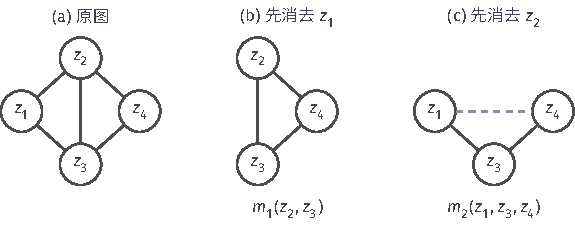
\includegraphics[width=97.282mm]{figures/01-mathematical-preliminaries-upper/05-graphs-and-signals/tikz/graph-theory-elimination-fill/figure.pdf}
  \caption{两个首步消元产生不同接口。删去$z_1$后新表索引$(z_2,z_3)$；
  删去$z_2$后通常须索引$(z_1,z_3,z_4)$，紫虚线为填充边$1-4$。
  二值稠密接口表分别有$4$和$8$项。特殊函数可能还能分解，图给出的是通用作用域上限。}
  \label{fig:graph-theory-elimination-fill}
\end{figure}

\paragraph{结构代价与后续表计算}
令$d_t$为第$t$步的剩余邻居数，补边候选对共$\sum_t d_t(d_t-1)/2$，袋记录量为$\sum_t(d_t+1)$。
支持期望常数查边与更新的哈希邻接集合下，给定次序的结构操作期望时间约为
$O(n+m+\sum_t d_t^2)$，存储含原边、$F$条填充边及全部袋；稠密矩阵则占$O(n^2)$。
每变量至多$q$状态时，处理一袋的稠密表至多$q^{k_\pi+1}$项，输出接口表至多$q^{k_\pi}$项，
总时间还取决于袋数、因子数与每次运算成本。结构操作数与数值表的指数代价要分别报告。
树宽恰等于最优消元诱导宽度的完整双向证明不在本节展开；
实践中最小度、最少填充等启发式只给出可计算的上界。

\subsection{基于贪心次序选择的补边分解法}

没有给定$\pi$时，可以每轮先按某个局部评分选下一个点，再调用同一套补边、记袋、删除步骤。
\paragraph{用当前局部代价选下一点}
最小度规则比较当前剩余邻居数，最少填充规则比较该邻域中还缺多少对边，二者是不同评分。
\begin{algorithm}[贪心消元次序]
  对当前全部活跃点计算所选评分，以固定编号打破平局，取最低分点记入$\pi$并执行补边删除，
  然后在更新后的图上重新评分，直到图空。
\end{algorithm}
不能把按初始度数排一次序当作动态最小度，也不能用原图缺边数代替当前缺边数。

\paragraph{局部选择数例与代价边界}
贯穿图中$1,4$的度为$2$、填充评分为$0$，$2,3$的度为$3$且缺边$1-4$、评分$1$，
按编号先选$1$；余下$\{2,3,4\}$成团，再按编号得$(1,2,3,4)$，构造宽度仍为$2$。
每轮重算全部评分的直接版本，检查量可达$\sum_t\sum_{v\text{活跃}}(1+d_t(v)^2)$、最坏约$O(n^4)$；
采用缓存或优先队列前必须说明哪些边增删触发重算。局部评分没有最优树宽保证。

\section{弦图条件下的团树构造法}
\label{sec:graph-theory-chordal-elimination}

本节希望直接用原图的极大团作袋。先把极大团、弦图、完美消元序和团树分别讲清，
再给出无填充次序的构造与极大团的连接方法。

\subsection{极大团、弦图与团树的基本概念}

\paragraph{团、极大团与最大团}
一个团若不能再加入图中其他顶点而仍保持两两相邻，称为\term{极大团}；
“极大”按集合包含判断，要检查能否继续扩张，不是先比较大小。
顶点数在全部团中最多的称\term{最大团}。例如三角形$1,2,3$外加边$3-4$，
极大团是$\{1,2,3\}$和$\{3,4\}$，后者虽不可扩张却比前者小，不是最大团。
贯穿图的两个三点极大团$\{1,2,3\},\{2,3,4\}$恰好也都是最大团，但这只是特例；
团树方法需要全部极大团，不能只取最大的几个。

\paragraph{弦、弦图与弦化}
长度至少$4$的环上，连接两个在环上不相邻顶点的边称为该环的\term{弦}（chord），
按环上位置判断而不按画线内外判断。每个长度至少$4$的环都有弦的有限无向图称\term{弦图}
（chordal graph）；树没有环因而也是弦图，无对角边的四环不是弦图。
弦图的诱导子图仍是弦图。给原图补边直到成为弦图称\term{弦化}（chordal completion），
它改变输入图、可能改变原分离关系，补全图上的团树不等价于原图的全部查询。

\paragraph{单纯顶点与完美消元序}
当前邻居已经两两相邻的顶点称\term{单纯顶点}（simplicial vertex），删除它无需补边；
空邻域和单点邻域也算单纯，且必须检查当前余图而非初始邻域。
若按一个完整次序删点时每步的待删点在当前余图中都单纯，该次序称\term{完美消元序}
（perfect elimination ordering）。
\begin{definition}[弦图与完美消元序]
  \label{def:graph-theory-chordal-graph}
  有限无向图是弦图，当且仅当它具有完美消元序。
\end{definition}
其依据有两方面：每个非空有限弦图都有单纯顶点（非完全弦图甚至有两个不相邻的单纯顶点），
删去单纯点后诱导余图仍是弦图，故可反复删到图空；反之，若有无弦长环，
环上最早删除的点面对两个尚不相临的环邻居，不可能单纯，矛盾。
存在好次序不等于任意次序都好：贯穿图本是弦图，但先删$2$时其剩余邻居$1,3,4$不两两相邻，仍须补$1-4$。

\paragraph{团树}
以原图全部极大团为袋并满足运行交集的袋树称\term{团树}（clique tree）。
相邻团的交集保存共同变量：贯穿图两个极大团交集为$\{2,3\}$，团树边承载两变量接口，
但团树不决定接口表上做加法、取最大还是其他运算。图不连通时，不同分量的团可用空交集边接成一棵树。
有限非空弦图能由全部极大团构成团树，非弦图则不能无条件照搬这套原团构造。

\subsection{基于单纯顶点删除的完美序构造法}

\paragraph{无填充删除的思想}
与允许补边的消元不同，这里只选择当前邻居已经成团的点，因而全程不扩大剩余连接；
目标是输出一个完整无填充次序，或指出图不满足弦图条件。
状态为当前活跃点集、当前邻接和已输出次序，单纯性在每次删除后重新检查。

\begin{algorithm}[单纯顶点删除构造完美序]
  在当前活跃点中按固定编号找候选$v$，枚举其不同邻居$u,w$确认每对之间都有边
  （空邻域、单邻居直接合格）；找到合格点就追加到次序、保存当前邻域并删除$v$及关联边，
  在余图上重复直到图空。若非空余图找不到单纯点，返回“不满足弦图条件”及该余图，不暗中补边。
\end{algorithm}

\paragraph{四环补弦的算例核验}
对四环$1-2-3-4-1$，每个点的两个邻居都不相邻（$1,3$看到$\{2,4\}$缺边$2-4$，
$2,4$看到$\{1,3\}$缺边$1-3$），没有合格点，方法返回失败。
补入弦$1-3$后，$2$的邻居$\{1,3\}$已相连；删$2$后$1$的邻居$\{3,4\}$相连，再删$1$，
随后依次删$3,4$，得到$(2,1,3,4)$且全程无新增边。

\paragraph{输出次序的独立核验}
\begin{algorithm}[完美消元序核验]
  独立于构造过程，给原图和待检次序：先确认次序长度为$n$且恰含每个顶点一次；
  建立每点rank，对每个$v$取出原图中排名更晚的邻居$N^+_\pi(v)$，逐对检查其间是否有原边，全程不补边。
  发现缺边即返回$v$与该缺边对作为失败见证；全部通过才认证为完美消元序。
\end{algorithm}
复查$(2,1,3,4)$用于无弦四环时，首点$2$的更晚邻居$\{1,3\}$缺边，立即拒绝；
用于已补$1-3$的图才通过。直接重查的朴素构造邻接检查量最坏约$O(n^4)$、稠密存邻接占$O(n^2)$；
独立核验建rank与读邻接为$O(n+m)$，邻居对检查数为
$\sum_v|N^+_\pi(v)|(|N^+_\pi(v)|-1)/2$。两者职责不同，不应混为一项代价。

\subsection{基于团交集最大权树的接口构造法}

\paragraph{以共享变量连接团的思想}
输入弦图和已核验的完美序，要输出以全部极大团为袋、满足运行交集的接口树。
直觉上交集大的团应相连以携带更多共享变量，但任意接线不一定满足运行交集，
需要一条明确的最大总交集权规则。

\paragraph{从完美序生成极大团列表}
对每点生成$K_v=\{v\}\cup N^+_\pi(v)$，完美序保证各$K_v$是团；
删除重复集合和被其他$K$严格包含的集合，得到全部极大团。不遗漏的原因是：
任一团取其中最早消去的点，其余点都在该点剩余邻域中，整个团包含于某个$K_v$，
而各$K_v$本身是团，极大者恰为极大团。

\paragraph{建立交集权并选树边}
在$p$个团节点上建完全候选图，边权取$w(C,D)=|C\cap D|$，交集为空的零权边也保留。
\begin{algorithm}[最大交集权团树]
  把候选边按交集权从大到小排序，用并查集只接纳连接两个不同当前团分量的边，
  接满$p-1$条即停止（$p=1$时返回单个袋）；树边同时记录实际的接口集合。
\end{algorithm}
这与第15章的最大权生成树是同一种选边机制，其交换正确性在该章统一分析。

\begin{theorem}[最大权生成树与团树]
  \label{thm:graph-theory-clique-tree-maximum-weight}
  设$\mathcal H$为非空有限弦图，$\mathcal C$为其全部极大团，在以$\mathcal C$为节点的完全图上
  令$w(C,D)=|C\cap D|$（含零权边）。则候选图的一棵生成树满足运行交集，
  当且仅当它的总交集权最大。
\end{theorem}
直观理由是：对每个原顶点$v$，含$v$的$k_v$个团节点在树上至多需要$k_v-1$条两端含$v$的边
就能连成一片，等号成立恰当这些团连通；把所有顶点的这份计数相加就是总交集权，
而完美序构造出的团树能对每个顶点取等号，故最大权树恰满足运行交集。

\paragraph{贯穿图及四环的算例核验}
贯穿图极大团为$\{1,2,3\},\{2,3,4\}$，唯一候选边权$2$、接口$\{2,3\}$，
$2,3$在两端且经含它们的边相连。四环的极大团只是四条原边，
若要让每个顶点所属的两个边团都直接相连就需要四条连接而成环，选不出树，
所以不能给非弦四环的原团列表随便选一棵最大权树就宣称满足运行交集。
给定弦图上连接团、为原图选弦化、在所有补边中找最小宽度是三件不同的任务；
交集权计算、排序及包含筛选的代价也要随团数与集合表示另行计入。

\section{基于祖先道德化的d-分离判定法}
\label{sec:graph-theory-directed-transformations}

第13章定义了活跃路径与d-分离，但逐条枚举全部底层路径代价高且容易遗漏。
本节把一次条件分离查询等价地转换成一张临时无向图上的可达查询。

\paragraph{条件分离查询的输入与\term{祖先闭包}}
输入有限DAG和两两不交、$A,B$非空的集合$A,B,S$，判定给定$S$时$A,B$是否d-分离。
集合$W$的祖先闭包
\[
  \operatorname{An}(W)=W\cup\{v:\text{存在从}v\text{到}W\text{中某点的有向路径}\}
\]
显式包含$W$自身；本次查询取$W=A\cup B\cup S$。祖先闭包要在入邻接表上逆向BFS/DFS求得。

\paragraph{诱导\term{祖先图}、骨架与\term{道德图}}
在祖先闭包$U$上取诱导图$\mathcal G[U]$，保留$U$内部全部原弧——先限定点集再补边，
次序不可交换。有向图的骨架只是去掉弧方向、保留原有邻接。
\term{道德化}（moralization）则先把每个顶点的不同父节点两两相连、再去掉全部方向，
新增的父点边是它与骨架的区别；这里只对诱导祖先图道德化。

\begin{definition}[骨架、祖先闭包与道德图]
  \label{def:graph-theory-directed-structure}
  骨架$\operatorname{skel}(\mathcal G)$是同顶点集的无向图，$i,j$相邻当且仅当
  $i\to j$或$j\to i$存在。祖先闭包$\operatorname{An}(W)$如上定义，
  $\mathcal G[\operatorname{An}(W)]$为诱导祖先图。道德图$\operatorname{mor}(\mathcal G)$
  把每个顶点的任意两个不同父节点连成无向边后再去掉所有弧方向；
  若每个父集在骨架中原本已两两相邻，称该DAG为\term{完美有向图}。
\end{definition}

\paragraph{逆向检索到无向分隔的五步实现}
\begin{algorithm}[祖先道德化d-分离判定]
  第一步，以$A\cup B\cup S$为多源在入邻接表上逆向遍历，得到祖先闭包$U$（保留种子本身）；
  第二步取诱导图$\mathcal G[U]$；第三步只在该诱导图内，把每个顶点的父集无序对补边并去掉全部方向，
  得到本次查询的无向道德图；第四步删除$S$及关联边；第五步从$A$的所有点同时BFS，
  检查能否到达$B$：能到达则不d-分离，否则d-分离，并可沿前驱输出查询图中的一条路径。
\end{algorithm}
其等价性依据是：给定$S$时原图的一条活跃路径，其碰撞点都在$S$的祖先中、
其余内部点都是端点或$S$的祖先，故整条路径落在诱导祖先图里，
用道德边绕过属于$S$的碰撞点便得到避开$S$的无向路径；反过来，道德图中避开$S$的路径
把每条新增道德边展开回$u\to c\leftarrow v$，必要时沿有向路径改道，也能还原出一条活跃路径。
这里只使用该判据与操作次序，完整的路线去重证明不在主线展开。查询图里沿道德边走的路线
不是原图中顺箭头的有向路径。

\begin{figure}[htbp]
  \centering
  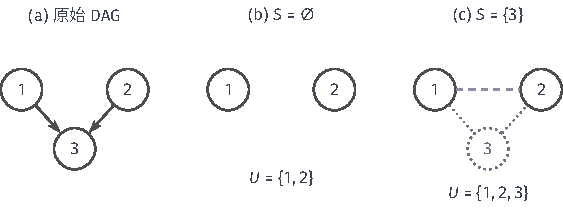
\includegraphics[width=95.282mm]{figures/01-mathematical-preliminaries-upper/05-graphs-and-signals/tikz/graph-theory-ancestor-moral-query/figure.pdf}
  \caption{祖先道德图随查询条件改变。端点固定为$1,2$；空条件集时查询图只有两个孤立顶点。
  给定$3$时，扩大的祖先集合使道德化加入新增边$1-2$，删除条件点$3$后这条边仍在。
  不能先道德化整图再取查询顶点。}
  \label{fig:graph-theory-ancestor-moral-query}
\end{figure}

\paragraph{碰撞及另一条通路的逐步查询}
如图~\ref{fig:graph-theory-ancestor-moral-query}，在$1\to3\leftarrow2$上取$A=\{1\},B=\{2\}$：
空条件时祖先闭包只有$\{1,2\}$，诱导图没有$3$、不补$1-2$，两点不连通，判为d-分离；
$S=\{3\}$时闭包含三点，父集$\{1,2\}$促使道德化补$1-2$，删$3$后边仍在，判为不分离。
若另有$3\to d$，给定后代$d$也会经祖先闭包得到同样结果。若先对整图道德化再截取$\{1,2\}$，
会错误留下$1-2$，说明“先取祖先、后道德化”的次序不能交换。
此外即使碰撞路径在空条件下关闭，若另有链$a\to e\to b$，$a,b$仍不分离：
阻断一条路径不足以确认分离。

\paragraph{代价、表示与查询边界}
建入邻接与逆向祖先检索为$O(n+a)$。道德化要枚举诱导图中每个父集的点对，
共$\sum_v p_v(p_v-1)/2$对，点的父集很大时即使原图稀疏、查询图也可能接近稠密，
不能把整步统称$O(n+a)$；用稠密掩码存边另占$O(n^2)$。每次$A,B,S$变化都可能改变祖先集和新增边，
输出的是这一次查询的临时等价无向图，不自动给出一张保留全部条件查询的固定图，
从图分离到概率独立仍需第13章说明的分解假设。

\section{本章小结}

\paragraph{访问次序与查询输出}
BFS给出边数层和一条发现路线，DFS给出当前分支、回边见证与完成信息；
Kahn与DFS逆完成序在DAG上构造处理次序。需要什么输出决定保存什么状态，
任一遍历次序都不能直接当作最短路线或拓扑序。连通标记、两遍标签合并和种子队列重建
复用同一套邻接检索，但分别输出全部分量或指定可达集，$4/8$邻接、掩模范围、
结构元方向和空种子条件都随方法固定。

\paragraph{分解的作用与代价}
父边提取保留分量连通却可能改变距离和分隔；给定分隔集把共享变量保留为接口，
消元补边再把潜在作用域组织成袋，宽度控制同时索引的变量数。
运行交集约束变量取值能否沿接口核对，因子唯一归属约束数值不被重复计入，二者缺一不可。
次序会改变填充与最大袋规模；单纯顶点删除在弦图条件下给无填充记录，
团交集最大权树再连接全部极大团，它们都有具体输入与构造代价，不因其名称就成为线性或最优。

\paragraph{单次分离查询与后续计算}
祖先道德化按“逆向求祖先—取诱导图—补父点边—删条件点—无向检索”五步完成一次d-分离判定，
查询图随$A,B,S$而变。本章产出的是访问次序、标签、连接骨架、局部袋和判定结果；
第15章在相应结构上加入路径、流量、生成树等优化目标，第16章在合法运算下组合、汇总配置表。
结构可用、目标最优与数值查询正确，是需要分别建立的三件事。
